\documentclass{standalone}

\usepackage{tikz}

\definecolor{myBlue}{RGB}{15,158,213}
\definecolor{myPurple}{RGB}{160,43,147}
\definecolor{myOrange}{RGB}{233,113,50}

\begin{document}
	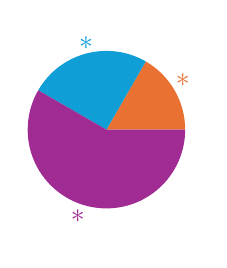
\begin{tikzpicture}
		\fill[myOrange] (0,0) -- (0:1) arc (0:60:1) node[midway,above,xshift=3pt,yshift=-5pt] {*} -- cycle;
	    \fill[myBlue] (0,0) -- (60:1) arc (60:150:1) node[midway,above,yshift=-5pt] {*} -- cycle;
	    \fill[myPurple] (0,0) -- (0:1) arc (0:-210:1) node[midway,below,xshift=-3pt,yshift=2pt] {*} -- cycle;
	\end{tikzpicture}
\end{document}
